% Comparison of the Chapter 3 method and the Appendix E router (SNR_R).
% Standalone; compile with pdflatex (twice).
\documentclass[11pt,a4paper]{article}
\usepackage[margin=2.2cm]{geometry}
\usepackage[T1]{fontenc}
\usepackage{lmodern}
\usepackage{microtype}
\usepackage{booktabs,tabularx,array}
\usepackage{enumitem}
\usepackage{amssymb}
\usepackage{xcolor}
\usepackage{tikz}
\usetikzlibrary{arrows.meta,positioning,shapes.geometric}
\usepackage[hidelinks]{hyperref}
\newcolumntype{L}{>{\raggedright\arraybackslash}X}
\newcolumntype{P}[1]{>{\raggedright\arraybackslash}p{#1}}
\setlist{itemsep=2pt,topsep=3pt}
\setlength{\parskip}{4pt}
\setlength{\parindent}{0pt}
\definecolor{accent}{RGB}{0,90,170}
\newcommand{\snrr}{\texttt{SNR\_R}}

\title{\textbf{Current Method vs.\ Appendix E Router}\\[2pt]\large Comparison, Suitability and Action Points}
\author{Prepared for Mark Vincent D.\ Limpahan and the thesis group}
\date{18 November 2026}

\setlength{\tabcolsep}{4pt}
\begin{document}
\maketitle

\noindent\textit{Basis:} Chapter~3 and Appendices~D and~E of the manuscript as of 18 Nov 2026 (GitHub \texttt{main}, commit \texttt{b3042cb}). Section, table and appendix numbers refer to that manuscript.

% ---------------------------------------------------------------------
\section{Bottom Line}

The Appendix~E router (\snrr) is worth pursuing, but it is not ready to replace the Chapter~3 method in the manuscript yet. On 30 development speakers it beat the Chapter~3 reference by $+0.58$ UTMOS at 13 instead of 21 forward passes, while the Chapter~3 stopping rule failed its own audit (no certified saving across six noise levels).

Three things block a straight swap: its thresholds are not calibrated with Learn-Then-Test, it has not been run on held-out speakers, and its advantage over the cheaper teacher-free option (\texttt{STUR2}, 3 passes) rests on prosodic diversity, which Chapter~1 (Section~1.5) currently puts out of scope.

\textbf{Recommended path:} adopt \snrr{} as the proposed method only with the adviser's agreement, keep the Chapter~3 stopping-time rule as a compared baseline, bring diversity into scope as a secondary measure, and calibrate the residual threshold with Learn-Then-Test before the manuscript claims a guarantee.

% ---------------------------------------------------------------------
\section{The Two Methods Side by Side}

The current method decides \emph{when} the teacher stops; the Appendix~E router always stops at one point and decides \emph{what} the teacher hands over (Figure~\ref{fig:compare}, Table~\ref{tab:side}).

\begin{figure}[!htbp]
\centering
\resizebox{\textwidth}{!}{%
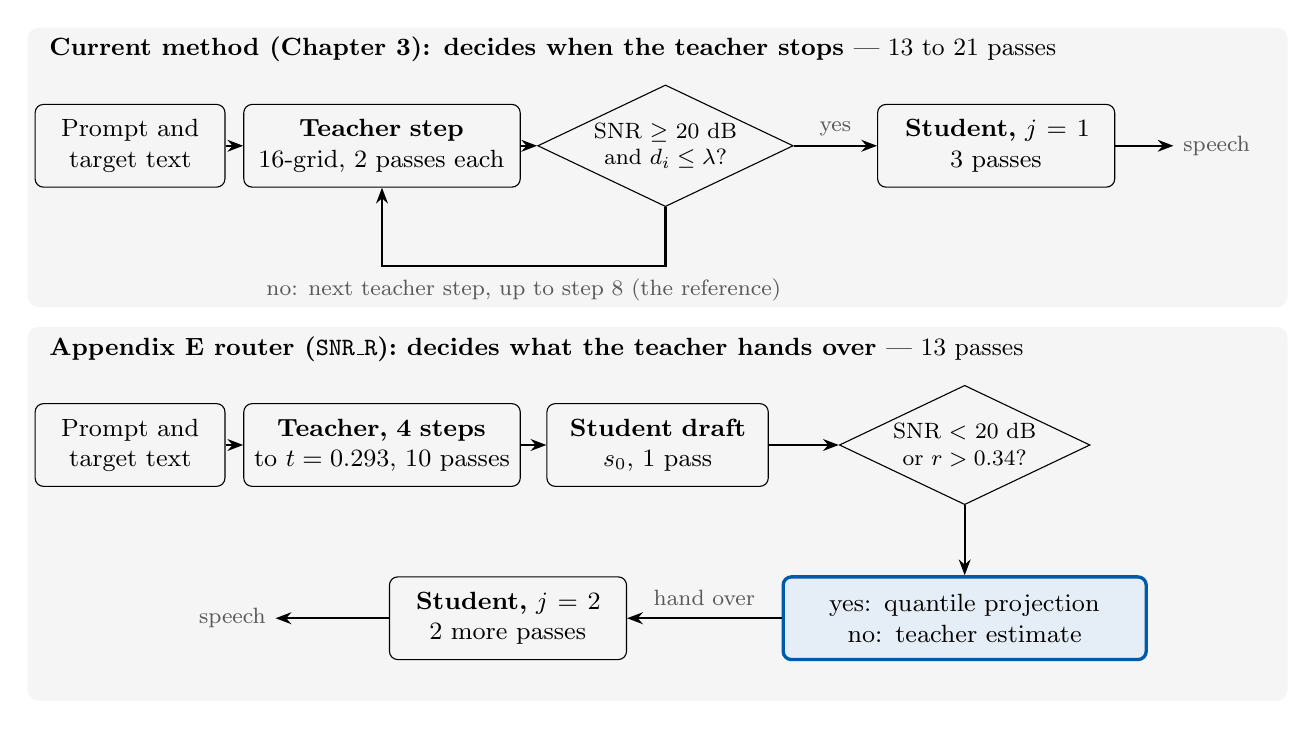
\begin{tikzpicture}[
  font=\small,
  box/.style={draw, rounded corners=3pt, align=center, minimum height=1.05cm, inner sep=3pt},
  key/.style={box, draw=accent, very thick, fill=accent!10},
  dec/.style={diamond, draw, aspect=2.1, align=center, inner sep=1pt, font=\footnotesize},
  arr/.style={-{Stealth[length=2mm]}, thick},
  lab/.style={font=\footnotesize, text=black!65},
  lane/.style={font=\small\bfseries, anchor=west}
]
% lane 1
\fill[black!4, rounded corners=4pt] (-0.6,1.0) rectangle (15.4,-2.55);
\node[lane] at (-0.45,0.72) {Current method (Chapter 3): decides when the teacher stops \textnormal{--- 13 to 21 passes}};
\node[box, text width=2.2cm] (ci) at (0.7,-0.5) {Prompt and\\target text};
\node[box, text width=3.3cm] (ct) at (3.9,-0.5) {\textbf{Teacher step}\\16-grid, 2 passes each};
\node[dec] (cd) at (7.5,-0.5) {SNR $\ge$ 20 dB\\and $d_i\le\lambda$?};
\node[box, text width=2.8cm] (cs) at (11.7,-0.5) {\textbf{Student, $j=1$}\\3 passes};
\node[lab] (csp) at (14.5,-0.5) {speech};
\draw[arr] (ci) -- (ct); \draw[arr] (ct) -- (cd);
\draw[arr] (cd) -- node[lab, above] {yes} (cs);
\draw[arr] (cs) -- (csp);
\draw[arr] (cd.south) -- ++(0,-0.75) -| node[lab, pos=0.25, below=1pt] {no: next teacher step, up to step 8 (the reference)} (ct.south);
% lane 2
\fill[black!4, rounded corners=4pt] (-0.6,-2.8) rectangle (15.4,-7.55);
\node[lane] at (-0.45,-3.08) {Appendix E router (\snrr): decides what the teacher hands over \textnormal{--- 13 passes}};
\node[box, text width=2.2cm] (ei) at (0.7,-4.3) {Prompt and\\target text};
\node[box, text width=3.3cm] (et) at (3.9,-4.3) {\textbf{Teacher, 4 steps}\\to $t=0.293$, 10 passes};
\node[box, text width=2.6cm] (ed) at (7.4,-4.3) {\textbf{Student draft}\\$s_0$, 1 pass};
\node[dec] (edc) at (11.3,-4.3) {SNR $<$ 20 dB\\or $r>0.34$?};
\node[key, text width=4.4cm] (ep) at (11.3,-6.5) {yes: quantile projection\\no: teacher estimate};
\node[box, text width=2.8cm] (es) at (5.5,-6.5) {\textbf{Student, $j=2$}\\2 more passes};
\node[lab] (esp) at (2.0,-6.5) {speech};
\draw[arr] (ei) -- (et); \draw[arr] (et) -- (ed); \draw[arr] (ed) -- (edc);
\draw[arr] (edc) -- (ep);
\draw[arr] (ep) -- node[lab, above=1pt] {hand over} (es);
\draw[arr] (es) -- (esp);
\end{tikzpicture}}
\caption{Both methods use the same frozen teacher (F5-TTS) and student (DMOSpeech~2); only the point of decision and its object differ. The highlighted box is the router's per-utterance choice of payload.}
\label{fig:compare}
\end{figure}

\begin{table}[!htbp]
\centering\small
\caption{The two methods compared attribute by attribute.}
\label{tab:side}
\begin{tabularx}{\textwidth}{@{}P{3.1cm} L L@{}}
\toprule
& \textbf{Current method (Chapter 3)} & \textbf{Appendix E router (\snrr)} \\
\midrule
Per-utterance decision & Teacher stopping step, chosen among steps 4 to 8 & Handover payload: teacher estimate (\texttt{CPH8}) or its quantile projection (\texttt{CPQH}) \\
Teacher grid and stop & 16-interval sway grid; stops between $t=0.076$ and $0.293$ & 8-interval sway grid; always stops at $t=0.2929$ (10 teacher passes) \\
Student restart & $j=1$ ($\tau=0.0761$), 3 student passes & One-pass student draft, then $j=2$, 2 more student passes \\
Decision signals & Prompt SNR gate (20 dB) and endpoint-stabilization score $d_i$ & Prompt SNR gate (20 dB) and invariant residual $r$ between teacher estimate and student draft \\
Rule & Stop at the first candidate with SNR $\ge 20$ dB and $d_i\le\lambda$; otherwise the reference (Definition~3.4) & Use \texttt{CPQH} when SNR $<20$ dB or $r>0.34$; otherwise \texttt{CPH8} \\
Cost per utterance & 13 to 21 forward passes, varies by utterance & 13 forward passes, fixed (12 for SNR-only routing) \\
Threshold setting & Learn-Then-Test on 200 calibration speakers, with a stated bound on added failures & Fixed from a 12-sentence CPU screen; no Learn-Then-Test yet \\
Theory & Six propositions: cost, zero overhead, monotone cost, safe fallback, oracle bound, LTT guarantee & Three propositions: invariance of $Q$, zero residual under time rearrangement, residual equals Wasserstein-2 energy \\
Optimizes & Fewest passes subject to an added-failure limit & Best quality at a fixed low cost, keeping clean prosodic variety \\
Weights changed & None & None \\
\bottomrule
\end{tabularx}
\end{table}

The key difference for the thesis is the objective. Chapter~3 trades quality for cost under a risk limit; \snrr{} fixes the cost at about 62\% of the reference and spends its decision on robustness to degraded prompts.

% ---------------------------------------------------------------------
\section{What the Evidence Says}

The Chapter~3 rule works on clean versus 15 dB prompts but fails once intermediate noise enters; \snrr{} fixes exactly that failure, on development data only.

\subsection*{Current method (Appendix D)}
\begin{itemize}[leftmargin=1.3em]
\item On 200 development instances (clean and 15 dB), cross-validation saved 10.1\% of passes with 1 added failure, and 27\% of clean synthesis time.
\item Across six noise levels, Learn-Then-Test certified no threshold for the $d_i$ rule: 0.0\% saving on the 16-interval grid (1.8\% on the 32-interval grid).
\item Noise makes $d_i$ smaller (median 0.61 clean, 0.17 at 15 dB), so noisy prompts look settled first and would be handed over first.
\item The 20 dB SNR gate lets 18 to 22 dB noise through (23.9\% added failures) and reads telephone audio as 44 dB.
\item Two references of equal quality disagree on 22.5\% of binary failure labels from student randomness alone, so the failure rule itself is noisy.
\end{itemize}

\subsection*{Appendix E router (EXP-034)}
240 cases: 30 development speakers $\times$ 8 prompt conditions, on the Tesla T4 (Table~\ref{tab:evidence}).

\begin{table}[!htbp]
\centering\small
\caption{Quality and cost on the same 240 EXP-034 cases (Appendix E).}
\label{tab:evidence}
\begin{tabular}{@{}l r r r r r@{}}
\toprule
\textbf{Method} & \textbf{Passes} & \textbf{Clean time (s)} & \textbf{UTMOS} & \textbf{WER} & \textbf{SIM} \\
\midrule
\texttt{W8}, Chapter 3 reference & 21 & 3.41 & 2.368 & 0.054 & 0.859 \\
\texttt{SNR\_ONLY} routing & 12.3 & 1.94 & 2.376 & 0.048 & 0.868 \\
\textbf{\snrr, proposed} & \textbf{13} & \textbf{2.11} & \textbf{2.950} & \textbf{0.047} & \textbf{0.883} \\
\texttt{CPQH}, always & 13 & 2.12 & 2.963 & 0.048 & 0.885 \\
\texttt{STUR2}, no teacher & 3 & 0.51 & 3.114 & 0.031 & 0.884 \\
\bottomrule
\end{tabular}
\end{table}

\begin{itemize}[leftmargin=1.3em]
\item All five preregistered hypotheses passed. The residual $r$ detects cases that need \texttt{CPQH} with AUC 0.864, against 0.697 for $d_4$.
\item The gain comes from the 25 dB white, pink and high-pass conditions, where \snrr{} reaches 3.61 to 3.87 UTMOS and \texttt{SNR\_ONLY} 1.83 to 2.74.
\item On clean prompts \snrr{} keeps 96\% of the teacher's aligned pitch variety; always using \texttt{CPQH} keeps 87\%.
\end{itemize}

\subsection*{Limits of the Appendix E evidence}
\begin{itemize}[leftmargin=1.3em]
\item 30 development speakers, not the held-out test split; thresholds come from a CPU screen, with no risk certificate.
\item \texttt{STUR2} is better on UTMOS and WER, and level on SIM, at less than a quarter of the cost; the teacher only earns its place through prosodic variety.
\item \snrr{} and always-\texttt{CPQH} tie on quality at the same cost; the router's only edge is clean pitch variety (96\% vs.\ 87\%).
\item Every method stays poor on heavy reverberation (about 1.4 UTMOS) and telephone audio (about 1.5 to 1.6).
\end{itemize}

% ---------------------------------------------------------------------
\section{Is It Suitable to Pursue?}

Yes on evidence and novelty, but adopting it changes the thesis's objective and scope, so it needs the adviser's approval (Table~\ref{tab:suit}).

\begin{table}[!htbp]
\centering\small
\caption{Fit of each method with the thesis, the panel's comments and the timeline.}
\label{tab:suit}
\begin{tabularx}{\textwidth}{@{}P{3.0cm} L L L@{}}
\toprule
\textbf{Criterion} & \textbf{Current method} & \textbf{Appendix E router} & \textbf{What adopting it changes} \\
\midrule
Fits the title (risk-calibrated, adaptive handover, teacher-guided) & Fully & Adaptive and teacher-guided; not yet risk-calibrated & Calibrate $\lambda_r$ with Learn-Then-Test so the title still holds \\
Research questions and objectives & Written for it & Objective 1 (sweep of stopping times) and Objective 2 (fewest passes under a risk limit) no longer match & Rewrite the three questions around payload choice at a fixed low cost \\
Panel: lightweight, cost (items 13, 19) & 13 to 21 passes, varies & 13 passes, 38\% fewer than the reference & The saving becomes fixed, not per utterance \\
Panel: novelty (items 9, 22) & Weaker: AdaVLA and FlowGuard already use step-change signals & Stronger: no reviewed study hands over a quantile projection or uses an invariant residual & Chapter 2 needs work on quantile mapping and optimal transport \\
Panel: reusable threshold (items 20, 26) & Calibrated $\lambda$ & $\lambda_r$, if calibrated & Same claim, new threshold \\
Evidence & Fails the multi-noise audit & Passes all preregistered tests on development data & Needs a held-out run before the manuscript relies on it \\
Scope (Section 1.5) & Diversity not measured & Its case over \texttt{STUR2} rests on diversity & Bring pitch variety ($\mathrm{CV}_{f_0}$) in as a secondary measure \\
Workload before the defense & Text already written & Rewrite of Sections 3.5 to 3.7, plus parts of Chapters 1 and 2 & About as much writing as the post-concept revisions \\
\bottomrule
\end{tabularx}
\end{table}

The main risk of switching is the concept approval: the panel approved a stopping-time design on 27 Oct 2026, so a new method should be presented as an evidence-driven refinement, not a different study. The main risk of not switching is defending a rule that the team's own audit shows saves nothing across noise levels.

% ---------------------------------------------------------------------
\section{Options and Recommendation}

Option~C, a reframed study with \snrr{} as the proposed method and the stopping-time rule as a baseline, is the recommendation, subject to the adviser (Table~\ref{tab:options}).

\begin{table}[!htbp]
\centering\small
\caption{Three ways forward.}
\label{tab:options}
\begin{tabularx}{\textwidth}{@{}P{2.4cm} L L L@{}}
\toprule
\textbf{Option} & \textbf{What the manuscript says} & \textbf{Gains} & \textbf{Costs and risks} \\
\midrule
A.\ Keep Chapter 3 & The stopping-time rule stays the method; Appendices D and E are reported as risks and future work & Least rewriting; matches the approved concept & Defends a rule its own audit shows saves 0\% across noise levels; the panel may ask why the better router is not used \\
B.\ Replace with \snrr & Chapter 3 rewritten around the payload router only & Best development results; strongest novelty & Largest rewrite; looks like a new study; no LTT or held-out evidence yet \\
\textbf{C.\ Reframe (recommended)} & The per-utterance handover decision covers both when and what to hand over; \snrr{} is the proposed method, the stopping-time rule a compared baseline & Keeps the title and the concept's frame; uses the best evidence; the Chapter 3 work becomes the baseline, not wasted & Still a sizeable rewrite; needs LTT on $\lambda_r$ and diversity in scope \\
\bottomrule
\end{tabularx}
\end{table}

Under option~C the contribution reads: a training-free, risk-calibrated handover method for DMOSpeech~2 that, for each utterance, decides what the teacher hands to the student, with a Learn-Then-Test bound on added failures at a fixed cost of 13 passes. The stopping-time rule, \texttt{W8}, \texttt{STUR2} and always-\texttt{CPQH} become the compared methods, which also answers the panel's request for a comparison matrix.

Two questions decide whether option~C holds up: does \snrr{} keep its lead on held-out speakers once $\lambda_r$ is certified, and is prosodic variety a strong enough reason to prefer it over \texttt{STUR2}? If either answer is no, fall back to option~A with Appendix~E as future work.

% ---------------------------------------------------------------------
\section{Action Points}

The first step is a decision, not writing: take options A and C to the adviser with this comparison, then run the two confirming experiments before anyone rewrites Chapter~3.

\subsection*{Decisions for the group and adviser}
\begin{itemize}[label=$\square$, leftmargin=1.5em]
\item Option A or option C (or B).
\item Whether prosodic variety ($\mathrm{CV}_{f_0}$) enters the scope as a secondary measure.
\item Whether the failure rule stays binary (Definition~3.1) or adds paired TOST equivalence, given the 22.5\% label noise.
\item The moderate-noise level for the protocol (25 dB is where the router's gain lies).
\end{itemize}

\subsection*{Work if option C is chosen}
\begin{table}[!htbp]
\centering\small
\caption{Work plan under option C.}
\label{tab:actions}
\begin{tabularx}{\textwidth}{@{}r L P{2.0cm} P{2.9cm} P{1.6cm}@{}}
\toprule
\textbf{\#} & \textbf{Action} & \textbf{Owner} & \textbf{Where} & \textbf{Depends on} \\
\midrule
1 & Calibrate $\lambda_r$ with Learn-Then-Test on the calibration split and report the certified bound & Rhenel & Experiments; Section 3.7 & Decision \\
2 & Run \snrr, \texttt{W8}, the stopping-time rule, \texttt{STUR2} and always-\texttt{CPQH} on the held-out test split and on LibriSpeech-PC & Rhenel & Experiments; Section 3.8 & 1 \\
3 & Small listening check on clean and 25 dB outputs of \snrr, \texttt{STUR2} and \texttt{W8} & All & Appendix E & 2 \\
4 & Rewrite Sections 3.5 to 3.7 around the payload router; move Appendix E's definitions and three propositions into Chapter 3; keep the stopping-time rule as a baseline & Mark & Chapter 3 & Decision \\
5 & Update the comparison matrix (Table 3.9), workflow figure and cost table for the 8-interval grid and $j=2$ & Mark & Chapter 3 & 4 \\
6 & Rewrite the research questions, objectives, Sections 1.6 to 1.7 and the conceptual figure; add $\mathrm{CV}_{f_0}$ to scope & Mark, Roxanne & Chapter 1 & Decision \\
7 & Add related work on quantile mapping and histogram matching, optimal transport (Wasserstein-2) and invariance; update the synthesis table and gap & Art & Chapter 2 & Decision \\
8 & Reconcile Appendix D's summary table and Table C.1 with the chosen method; remove the unused \texttt{fig\_stac.tex} & Rhenel & Appendices C and D & 4 \\
9 & Update the revision matrix and regenerate the highlighted-revisions file & Mark & Revision matrix & 4 to 7 \\
\bottomrule
\end{tabularx}
\end{table}

\textbf{If option A is chosen instead:} keep Chapter~3, add one paragraph in Section~3.6 naming the audit results as known risks, move Appendix~E into future work, and fix the small leftovers (Table~3.9's Step~7 row, Table~3.4's LibriSpeech-PC row, the moderate-noise level).

\end{document}
